% Created by tikzDevice version 0.12.3.1 on 2021-06-29 20:57:30
% !TEX encoding = UTF-8 Unicode
´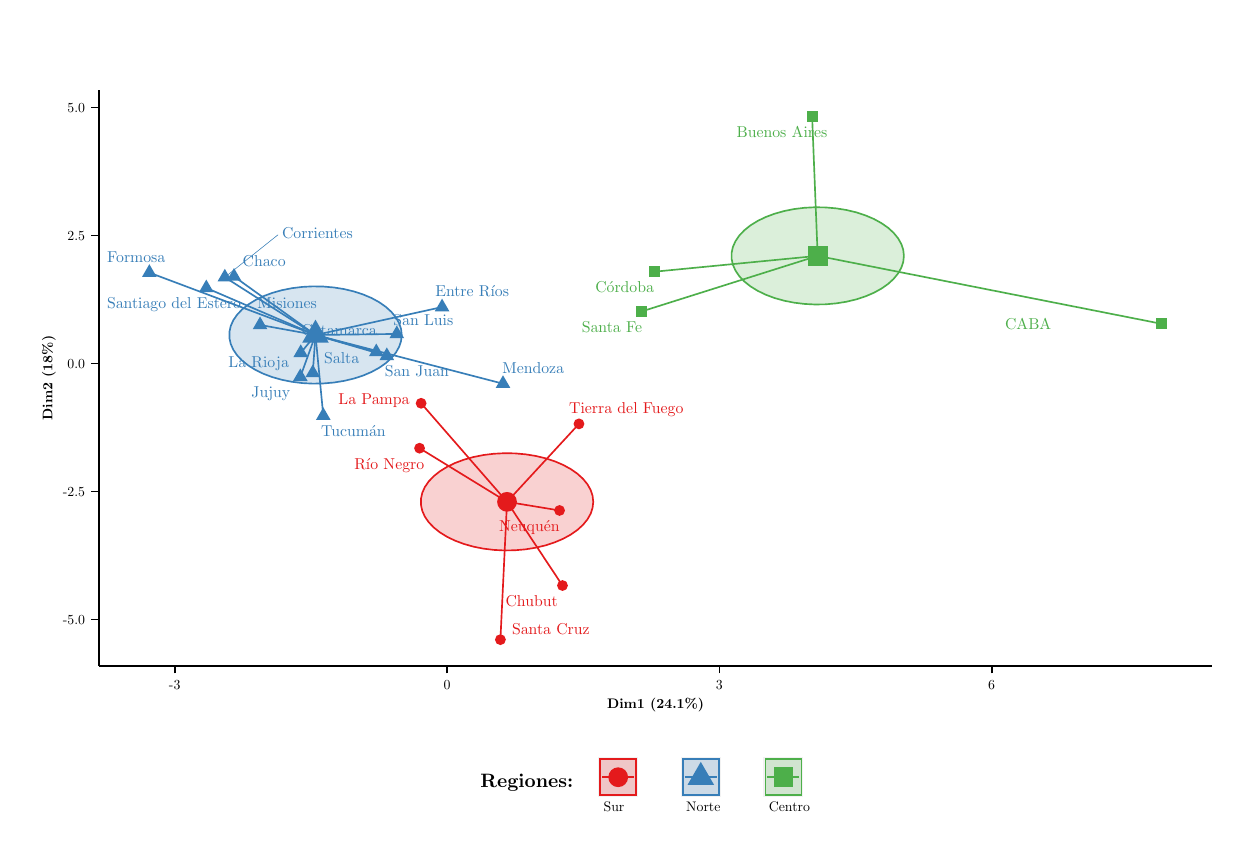
\begin{tikzpicture}[x=1pt,y=1pt]
\definecolor{fillColor}{RGB}{255,255,255}
\path[use as bounding box,fill=fillColor,fill opacity=0.00] (0,0) rectangle (433.62,289.08);
\begin{scope}
\path[clip] (  0.00,  0.00) rectangle (433.62,289.08);
\definecolor{drawColor}{RGB}{255,255,255}
\definecolor{fillColor}{RGB}{255,255,255}

\path[draw=drawColor,line width= 0.6pt,line join=round,line cap=round,fill=fillColor] (  0.00, -0.00) rectangle (433.62,289.08);
\end{scope}
\begin{scope}
\path[clip] ( 25.68, 58.49) rectangle (428.12,266.40);
\definecolor{drawColor}{RGB}{255,255,255}

\path[draw=drawColor,line width= 0.3pt,line join=round] ( 25.68, 98.33) --
	(428.12, 98.33);

\path[draw=drawColor,line width= 0.3pt,line join=round] ( 25.68,144.59) --
	(428.12,144.59);

\path[draw=drawColor,line width= 0.3pt,line join=round] ( 25.68,190.85) --
	(428.12,190.85);

\path[draw=drawColor,line width= 0.3pt,line join=round] ( 25.68,237.12) --
	(428.12,237.12);

\path[draw=drawColor,line width= 0.3pt,line join=round] (102.34, 58.49) --
	(102.34,266.40);

\path[draw=drawColor,line width= 0.3pt,line join=round] (200.75, 58.49) --
	(200.75,266.40);

\path[draw=drawColor,line width= 0.3pt,line join=round] (299.15, 58.49) --
	(299.15,266.40);

\path[draw=drawColor,line width= 0.3pt,line join=round] (397.55, 58.49) --
	(397.55,266.40);

\path[draw=drawColor,line width= 0.6pt,line join=round] ( 25.68, 75.19) --
	(428.12, 75.19);

\path[draw=drawColor,line width= 0.6pt,line join=round] ( 25.68,121.46) --
	(428.12,121.46);

\path[draw=drawColor,line width= 0.6pt,line join=round] ( 25.68,167.72) --
	(428.12,167.72);

\path[draw=drawColor,line width= 0.6pt,line join=round] ( 25.68,213.98) --
	(428.12,213.98);

\path[draw=drawColor,line width= 0.6pt,line join=round] ( 25.68,260.25) --
	(428.12,260.25);

\path[draw=drawColor,line width= 0.6pt,line join=round] ( 53.14, 58.49) --
	( 53.14,266.40);

\path[draw=drawColor,line width= 0.6pt,line join=round] (151.54, 58.49) --
	(151.54,266.40);

\path[draw=drawColor,line width= 0.6pt,line join=round] (249.95, 58.49) --
	(249.95,266.40);

\path[draw=drawColor,line width= 0.6pt,line join=round] (348.35, 58.49) --
	(348.35,266.40);
\definecolor{fillColor}{RGB}{77,175,74}

\path[fill=fillColor] (407.86,180.09) --
	(411.79,180.09) --
	(411.79,184.01) --
	(407.86,184.01) --
	cycle;

\path[fill=fillColor] (281.50,254.99) --
	(285.42,254.99) --
	(285.42,258.92) --
	(281.50,258.92) --
	cycle;
\definecolor{fillColor}{RGB}{55,126,184}

\path[fill=fillColor] (125.97,174.94) --
	(128.61,170.36) --
	(123.32,170.36) --
	cycle;

\path[fill=fillColor] ( 74.56,202.23) --
	( 77.20,197.65) --
	( 71.92,197.65) --
	cycle;
\definecolor{fillColor}{RGB}{228,26,28}

\path[fill=fillColor] (193.25, 87.50) circle (  1.96);
\definecolor{fillColor}{RGB}{77,175,74}

\path[fill=fillColor] (224.66,198.94) --
	(228.58,198.94) --
	(228.58,202.87) --
	(224.66,202.87) --
	cycle;
\definecolor{fillColor}{RGB}{55,126,184}

\path[fill=fillColor] ( 71.24,201.95) --
	( 73.88,197.38) --
	( 68.60,197.38) --
	cycle;

\path[fill=fillColor] (149.74,191.17) --
	(152.38,186.60) --
	(147.10,186.60) --
	cycle;

\path[fill=fillColor] ( 43.97,203.61) --
	( 46.61,199.04) --
	( 41.33,199.04) --
	cycle;

\path[fill=fillColor] ( 98.53,165.97) --
	(101.17,161.40) --
	( 95.88,161.40) --
	cycle;
\definecolor{fillColor}{RGB}{228,26,28}

\path[fill=fillColor] (142.17,153.35) circle (  1.96);
\definecolor{fillColor}{RGB}{55,126,184}

\path[fill=fillColor] ( 98.68,174.65) --
	(101.32,170.07) --
	( 96.04,170.07) --
	cycle;

\path[fill=fillColor] (171.76,163.48) --
	(174.41,158.90) --
	(169.12,158.90) --
	cycle;

\path[fill=fillColor] ( 83.97,184.71) --
	( 86.61,180.13) --
	( 81.33,180.13) --
	cycle;
\definecolor{fillColor}{RGB}{228,26,28}

\path[fill=fillColor] (192.19,114.62) circle (  1.96);

\path[fill=fillColor] (141.61,137.12) circle (  1.96);
\definecolor{fillColor}{RGB}{55,126,184}

\path[fill=fillColor] (103.02,167.38) --
	(105.66,162.80) --
	(100.38,162.80) --
	cycle;

\path[fill=fillColor] (129.78,173.54) --
	(132.42,168.96) --
	(127.14,168.96) --
	cycle;

\path[fill=fillColor] (133.39,181.46) --
	(136.03,176.88) --
	(130.74,176.88) --
	cycle;
\definecolor{fillColor}{RGB}{228,26,28}

\path[fill=fillColor] (170.82, 67.94) circle (  1.96);
\definecolor{fillColor}{RGB}{77,175,74}

\path[fill=fillColor] (219.97,184.60) --
	(223.90,184.60) --
	(223.90,188.53) --
	(219.97,188.53) --
	cycle;
\definecolor{fillColor}{RGB}{55,126,184}

\path[fill=fillColor] ( 64.55,198.07) --
	( 67.19,193.49) --
	( 61.91,193.49) --
	cycle;
\definecolor{fillColor}{RGB}{228,26,28}

\path[fill=fillColor] (199.21,145.91) circle (  1.96);
\definecolor{fillColor}{RGB}{55,126,184}

\path[fill=fillColor] (106.82,151.92) --
	(109.46,147.35) --
	(104.18,147.35) --
	cycle;
\definecolor{drawColor}{RGB}{228,26,28}
\definecolor{fillColor}{RGB}{228,26,28}

\path[draw=drawColor,line width= 0.6pt,line join=round,line cap=round,fill=fillColor,fill opacity=0.20] (204.37,117.74) --
	(204.13,119.90) --
	(203.43,122.03) --
	(202.27,124.09) --
	(200.66,126.06) --
	(198.64,127.90) --
	(196.24,129.58) --
	(193.48,131.09) --
	(190.42,132.40) --
	(187.10,133.48) --
	(183.57,134.32) --
	(179.88,134.91) --
	(176.08,135.25) --
	(172.25,135.31) --
	(168.43,135.11) --
	(164.68,134.65) --
	(161.06,133.93) --
	(157.63,132.97) --
	(154.43,131.77) --
	(151.52,130.36) --
	(148.93,128.76) --
	(146.72,127.00) --
	(144.90,125.09) --
	(143.51,123.07) --
	(142.58,120.97) --
	(142.11,118.82) --
	(142.11,116.66) --
	(142.58,114.51) --
	(143.51,112.41) --
	(144.90,110.39) --
	(146.72,108.49) --
	(148.93,106.72) --
	(151.52,105.12) --
	(154.43,103.71) --
	(157.63,102.52) --
	(161.06,101.55) --
	(164.68,100.83) --
	(168.43,100.37) --
	(172.25,100.17) --
	(176.08,100.24) --
	(179.88,100.57) --
	(183.57,101.16) --
	(187.10,102.00) --
	(190.42,103.09) --
	(193.48,104.39) --
	(196.24,105.90) --
	(198.64,107.58) --
	(200.66,109.42) --
	(202.27,111.39) --
	(203.43,113.45) --
	(204.13,115.58) --
	(204.37,117.74) --
	cycle;
\definecolor{drawColor}{RGB}{55,126,184}
\definecolor{fillColor}{RGB}{55,126,184}

\path[draw=drawColor,line width= 0.6pt,line join=round,line cap=round,fill=fillColor,fill opacity=0.20] (135.16,178.03) --
	(134.92,180.19) --
	(134.22,182.31) --
	(133.06,184.38) --
	(131.45,186.34) --
	(129.43,188.18) --
	(127.03,189.87) --
	(124.27,191.38) --
	(121.21,192.68) --
	(117.89,193.76) --
	(114.35,194.61) --
	(110.66,195.20) --
	(106.87,195.53) --
	(103.04,195.60) --
	( 99.22,195.40) --
	( 95.47,194.94) --
	( 91.85,194.22) --
	( 88.42,193.25) --
	( 85.22,192.06) --
	( 82.31,190.65) --
	( 79.72,189.05) --
	( 77.50,187.28) --
	( 75.69,185.37) --
	( 74.30,183.36) --
	( 73.37,181.26) --
	( 72.90,179.11) --
	( 72.90,176.94) --
	( 73.37,174.80) --
	( 74.30,172.70) --
	( 75.69,170.68) --
	( 77.50,168.77) --
	( 79.72,167.01) --
	( 82.31,165.41) --
	( 85.22,164.00) --
	( 88.42,162.80) --
	( 91.85,161.84) --
	( 95.47,161.12) --
	( 99.22,160.65) --
	(103.04,160.45) --
	(106.87,160.52) --
	(110.66,160.85) --
	(114.35,161.45) --
	(117.89,162.29) --
	(121.21,163.37) --
	(124.27,164.68) --
	(127.03,166.18) --
	(129.43,167.87) --
	(131.45,169.71) --
	(133.06,171.68) --
	(134.22,173.74) --
	(134.92,175.87) --
	(135.16,178.03) --
	cycle;
\definecolor{drawColor}{RGB}{77,175,74}
\definecolor{fillColor}{RGB}{77,175,74}

\path[draw=drawColor,line width= 0.6pt,line join=round,line cap=round,fill=fillColor,fill opacity=0.20] (316.62,206.62) --
	(316.39,208.78) --
	(315.68,210.91) --
	(314.52,212.97) --
	(312.91,214.94) --
	(310.90,216.78) --
	(308.49,218.46) --
	(305.74,219.97) --
	(302.67,221.27) --
	(299.35,222.36) --
	(295.82,223.20) --
	(292.13,223.79) --
	(288.34,224.12) --
	(284.50,224.19) --
	(280.68,223.99) --
	(276.93,223.53) --
	(273.32,222.81) --
	(269.88,221.84) --
	(266.68,220.65) --
	(263.77,219.24) --
	(261.18,217.64) --
	(258.97,215.87) --
	(257.15,213.97) --
	(255.77,211.95) --
	(254.83,209.85) --
	(254.36,207.70) --
	(254.36,205.54) --
	(254.83,203.39) --
	(255.77,201.29) --
	(257.15,199.27) --
	(258.97,197.36) --
	(261.18,195.60) --
	(263.77,194.00) --
	(266.68,192.59) --
	(269.88,191.39) --
	(273.32,190.43) --
	(276.93,189.71) --
	(280.68,189.25) --
	(284.50,189.05) --
	(288.34,189.11) --
	(292.13,189.45) --
	(295.82,190.04) --
	(299.35,190.88) --
	(302.67,191.96) --
	(305.74,193.27) --
	(308.49,194.78) --
	(310.90,196.46) --
	(312.91,198.30) --
	(314.52,200.27) --
	(315.68,202.33) --
	(316.39,204.46) --
	(316.62,206.62) --
	cycle;
\definecolor{fillColor}{RGB}{228,26,28}

\path[fill=fillColor] (173.21,117.74) circle (  3.57);
\definecolor{fillColor}{RGB}{55,126,184}

\path[fill=fillColor] (104.00,183.58) --
	(108.80,175.25) --
	( 99.19,175.25) --
	cycle;
\definecolor{fillColor}{RGB}{77,175,74}

\path[fill=fillColor] (281.89,203.05) --
	(289.03,203.05) --
	(289.03,210.19) --
	(281.89,210.19) --
	cycle;
\definecolor{drawColor}{RGB}{228,26,28}

\path[draw=drawColor,line width= 0.6pt,line join=round] (173.21,117.74) -- (193.25, 87.50);

\path[draw=drawColor,line width= 0.6pt,line join=round] (173.21,117.74) -- (142.17,153.35);

\path[draw=drawColor,line width= 0.6pt,line join=round] (173.21,117.74) -- (192.19,114.62);

\path[draw=drawColor,line width= 0.6pt,line join=round] (173.21,117.74) -- (141.61,137.12);

\path[draw=drawColor,line width= 0.6pt,line join=round] (173.21,117.74) -- (170.82, 67.94);

\path[draw=drawColor,line width= 0.6pt,line join=round] (173.21,117.74) -- (199.21,145.91);
\definecolor{drawColor}{RGB}{55,126,184}

\path[draw=drawColor,line width= 0.6pt,line join=round] (104.00,178.03) -- (125.97,171.89);

\path[draw=drawColor,line width= 0.6pt,line join=round] (104.00,178.03) -- ( 74.56,199.18);

\path[draw=drawColor,line width= 0.6pt,line join=round] (104.00,178.03) -- ( 71.24,198.90);

\path[draw=drawColor,line width= 0.6pt,line join=round] (104.00,178.03) -- (149.74,188.12);

\path[draw=drawColor,line width= 0.6pt,line join=round] (104.00,178.03) -- ( 43.97,200.56);

\path[draw=drawColor,line width= 0.6pt,line join=round] (104.00,178.03) -- ( 98.53,162.92);

\path[draw=drawColor,line width= 0.6pt,line join=round] (104.00,178.03) -- ( 98.68,171.60);

\path[draw=drawColor,line width= 0.6pt,line join=round] (104.00,178.03) -- (171.76,160.43);

\path[draw=drawColor,line width= 0.6pt,line join=round] (104.00,178.03) -- ( 83.97,181.66);

\path[draw=drawColor,line width= 0.6pt,line join=round] (104.00,178.03) -- (103.02,164.33);

\path[draw=drawColor,line width= 0.6pt,line join=round] (104.00,178.03) -- (129.78,170.49);

\path[draw=drawColor,line width= 0.6pt,line join=round] (104.00,178.03) -- (133.39,178.41);

\path[draw=drawColor,line width= 0.6pt,line join=round] (104.00,178.03) -- ( 64.55,195.02);

\path[draw=drawColor,line width= 0.6pt,line join=round] (104.00,178.03) -- (106.82,148.87);
\definecolor{drawColor}{RGB}{77,175,74}

\path[draw=drawColor,line width= 0.6pt,line join=round] (285.46,206.62) -- (409.83,182.05);

\path[draw=drawColor,line width= 0.6pt,line join=round] (285.46,206.62) -- (283.46,256.95);

\path[draw=drawColor,line width= 0.6pt,line join=round] (285.46,206.62) -- (226.62,200.91);

\path[draw=drawColor,line width= 0.6pt,line join=round] (285.46,206.62) -- (221.93,186.56);
\definecolor{drawColor}{RGB}{55,126,184}

\path[draw=drawColor,line width= 0.2pt,line join=round,line cap=round] ( 90.44,214.22) -- ( 71.92,199.44);
\definecolor{drawColor}{RGB}{77,175,74}

\node[text=drawColor,anchor=base,inner sep=0pt, outer sep=0pt, scale=  0.57] at (361.53,180.11) {CABA};

\node[text=drawColor,anchor=base,inner sep=0pt, outer sep=0pt, scale=  0.57] at (272.57,249.36) {Buenos Aires};
\definecolor{drawColor}{RGB}{55,126,184}

\node[text=drawColor,anchor=base,inner sep=0pt, outer sep=0pt, scale=  0.57] at (112.55,177.68) {Catamarca};

\node[text=drawColor,anchor=base,inner sep=0pt, outer sep=0pt, scale=  0.57] at ( 85.46,202.86) {Chaco};
\definecolor{drawColor}{RGB}{228,26,28}

\node[text=drawColor,anchor=base,inner sep=0pt, outer sep=0pt, scale=  0.57] at (182.11, 79.90) {Chubut};
\definecolor{drawColor}{RGB}{77,175,74}

\node[text=drawColor,anchor=base,inner sep=0pt, outer sep=0pt, scale=  0.57] at (215.72,193.32) {Córdoba};
\definecolor{drawColor}{RGB}{55,126,184}

\node[text=drawColor,anchor=base,inner sep=0pt, outer sep=0pt, scale=  0.57] at (104.70,212.78) {Corrientes};

\node[text=drawColor,anchor=base,inner sep=0pt, outer sep=0pt, scale=  0.57] at (160.62,191.79) {Entre Ríos};

\node[text=drawColor,anchor=base,inner sep=0pt, outer sep=0pt, scale=  0.57] at ( 39.23,204.22) {Formosa};

\node[text=drawColor,anchor=base,inner sep=0pt, outer sep=0pt, scale=  0.57] at ( 87.86,155.43) {Jujuy};
\definecolor{drawColor}{RGB}{228,26,28}

\node[text=drawColor,anchor=base,inner sep=0pt, outer sep=0pt, scale=  0.57] at (125.14,152.90) {La Pampa};
\definecolor{drawColor}{RGB}{55,126,184}

\node[text=drawColor,anchor=base,inner sep=0pt, outer sep=0pt, scale=  0.57] at ( 83.48,166.27) {La Rioja};

\node[text=drawColor,anchor=base,inner sep=0pt, outer sep=0pt, scale=  0.57] at (182.67,164.10) {Mendoza};

\node[text=drawColor,anchor=base,inner sep=0pt, outer sep=0pt, scale=  0.57] at ( 93.75,187.72) {Misiones};
\definecolor{drawColor}{RGB}{228,26,28}

\node[text=drawColor,anchor=base,inner sep=0pt, outer sep=0pt, scale=  0.57] at (181.29,107.03) {Neuquén};

\node[text=drawColor,anchor=base,inner sep=0pt, outer sep=0pt, scale=  0.57] at (130.68,129.50) {Río Negro};
\definecolor{drawColor}{RGB}{55,126,184}

\node[text=drawColor,anchor=base,inner sep=0pt, outer sep=0pt, scale=  0.57] at (113.46,167.66) {Salta};

\node[text=drawColor,anchor=base,inner sep=0pt, outer sep=0pt, scale=  0.57] at (140.65,162.92) {San Juan};

\node[text=drawColor,anchor=base,inner sep=0pt, outer sep=0pt, scale=  0.57] at (142.97,181.38) {San Luis};
\definecolor{drawColor}{RGB}{228,26,28}

\node[text=drawColor,anchor=base,inner sep=0pt, outer sep=0pt, scale=  0.57] at (189.05, 69.90) {Santa Cruz};
\definecolor{drawColor}{RGB}{77,175,74}

\node[text=drawColor,anchor=base,inner sep=0pt, outer sep=0pt, scale=  0.57] at (211.12,179.00) {Santa Fe};
\definecolor{drawColor}{RGB}{55,126,184}

\node[text=drawColor,anchor=base,inner sep=0pt, outer sep=0pt, scale=  0.57] at ( 52.89,187.44) {Santiago del Estero};
\definecolor{drawColor}{RGB}{228,26,28}

\node[text=drawColor,anchor=base,inner sep=0pt, outer sep=0pt, scale=  0.57] at (216.32,149.57) {Tierra del Fuego};
\definecolor{drawColor}{RGB}{55,126,184}

\node[text=drawColor,anchor=base,inner sep=0pt, outer sep=0pt, scale=  0.57] at (117.72,141.29) {Tucumán};
\end{scope}
\begin{scope}
\path[clip] (  0.00,  0.00) rectangle (433.62,289.08);
\definecolor{drawColor}{RGB}{0,0,0}

\path[draw=drawColor,line width= 0.6pt,line join=round] ( 25.68, 58.49) --
	( 25.68,266.40);
\end{scope}
\begin{scope}
\path[clip] (  0.00,  0.00) rectangle (433.62,289.08);
\definecolor{drawColor}{RGB}{0,0,0}

\node[text=drawColor,anchor=base east,inner sep=0pt, outer sep=0pt, scale=  0.50] at ( 20.73, 73.47) {-5.0};

\node[text=drawColor,anchor=base east,inner sep=0pt, outer sep=0pt, scale=  0.50] at ( 20.73,119.74) {-2.5};

\node[text=drawColor,anchor=base east,inner sep=0pt, outer sep=0pt, scale=  0.50] at ( 20.73,166.00) {0.0};

\node[text=drawColor,anchor=base east,inner sep=0pt, outer sep=0pt, scale=  0.50] at ( 20.73,212.26) {2.5};

\node[text=drawColor,anchor=base east,inner sep=0pt, outer sep=0pt, scale=  0.50] at ( 20.73,258.52) {5.0};
\end{scope}
\begin{scope}
\path[clip] (  0.00,  0.00) rectangle (433.62,289.08);
\definecolor{drawColor}{RGB}{0,0,0}

\path[draw=drawColor,line width= 0.6pt,line join=round] ( 22.93, 75.19) --
	( 25.68, 75.19);

\path[draw=drawColor,line width= 0.6pt,line join=round] ( 22.93,121.46) --
	( 25.68,121.46);

\path[draw=drawColor,line width= 0.6pt,line join=round] ( 22.93,167.72) --
	( 25.68,167.72);

\path[draw=drawColor,line width= 0.6pt,line join=round] ( 22.93,213.98) --
	( 25.68,213.98);

\path[draw=drawColor,line width= 0.6pt,line join=round] ( 22.93,260.25) --
	( 25.68,260.25);
\end{scope}
\begin{scope}
\path[clip] (  0.00,  0.00) rectangle (433.62,289.08);
\definecolor{drawColor}{RGB}{0,0,0}

\path[draw=drawColor,line width= 0.6pt,line join=round] ( 25.68, 58.49) --
	(428.12, 58.49);
\end{scope}
\begin{scope}
\path[clip] (  0.00,  0.00) rectangle (433.62,289.08);
\definecolor{drawColor}{RGB}{0,0,0}

\path[draw=drawColor,line width= 0.6pt,line join=round] ( 53.14, 55.74) --
	( 53.14, 58.49);

\path[draw=drawColor,line width= 0.6pt,line join=round] (151.54, 55.74) --
	(151.54, 58.49);

\path[draw=drawColor,line width= 0.6pt,line join=round] (249.95, 55.74) --
	(249.95, 58.49);

\path[draw=drawColor,line width= 0.6pt,line join=round] (348.35, 55.74) --
	(348.35, 58.49);
\end{scope}
\begin{scope}
\path[clip] (  0.00,  0.00) rectangle (433.62,289.08);
\definecolor{drawColor}{RGB}{0,0,0}

\node[text=drawColor,anchor=base,inner sep=0pt, outer sep=0pt, scale=  0.50] at ( 53.14, 50.10) {-3};

\node[text=drawColor,anchor=base,inner sep=0pt, outer sep=0pt, scale=  0.50] at (151.54, 50.10) {0};

\node[text=drawColor,anchor=base,inner sep=0pt, outer sep=0pt, scale=  0.50] at (249.95, 50.10) {3};

\node[text=drawColor,anchor=base,inner sep=0pt, outer sep=0pt, scale=  0.50] at (348.35, 50.10) {6};
\end{scope}
\begin{scope}
\path[clip] (  0.00,  0.00) rectangle (433.62,289.08);
\definecolor{drawColor}{RGB}{0,0,0}

\node[text=drawColor,anchor=base,inner sep=0pt, outer sep=0pt, scale=  0.50] at (226.90, 42.93) {\bfseries Dim1 (24.1{\%})};
\end{scope}
\begin{scope}
\path[clip] (  0.00,  0.00) rectangle (433.62,289.08);
\definecolor{drawColor}{RGB}{0,0,0}

\node[text=drawColor,rotate= 90.00,anchor=base,inner sep=0pt, outer sep=0pt, scale=  0.50] at (  8.95,162.45) {\bfseries Dim2 (18{\%})};
\end{scope}
\begin{scope}
\path[clip] (  0.00,  0.00) rectangle (433.62,289.08);
\definecolor{fillColor}{RGB}{255,255,255}

\path[fill=fillColor] (158.08,  5.50) rectangle (295.71, 30.95);
\end{scope}
\begin{scope}
\path[clip] (  0.00,  0.00) rectangle (433.62,289.08);
\definecolor{drawColor}{RGB}{0,0,0}

\node[text=drawColor,anchor=base west,inner sep=0pt, outer sep=0pt, scale=  0.7] at (163.58, 14.43) {\bfseries Regiones:};
\end{scope}
\begin{scope}
\path[clip] (  0.00,  0.00) rectangle (433.62,289.08);
\definecolor{fillColor}{gray}{0.95}

\path[fill=fillColor] (206.15, 11.00) rectangle (220.61, 25.45);
\end{scope}
\begin{scope}
\path[clip] (  0.00,  0.00) rectangle (433.62,289.08);
\definecolor{fillColor}{RGB}{228,26,28}

\path[fill=fillColor] (213.38, 18.23) circle (  1.96);
\end{scope}
\begin{scope}
\path[clip] (  0.00,  0.00) rectangle (433.62,289.08);
\definecolor{drawColor}{RGB}{228,26,28}
\definecolor{fillColor}{RGB}{228,26,28}

\path[draw=drawColor,line width= 0.6pt,line cap=rect,fill=fillColor,fill opacity=0.20] (206.87, 11.71) rectangle (219.90, 24.74);
\end{scope}
\begin{scope}
\path[clip] (  0.00,  0.00) rectangle (433.62,289.08);
\definecolor{fillColor}{RGB}{228,26,28}

\path[fill=fillColor] (213.38, 18.23) circle (  3.57);
\end{scope}
\begin{scope}
\path[clip] (  0.00,  0.00) rectangle (433.62,289.08);
\definecolor{drawColor}{RGB}{228,26,28}

\path[draw=drawColor,line width= 0.6pt,line join=round] (207.60, 18.23) -- (219.16, 18.23);
\end{scope}
\begin{scope}
\path[clip] (  0.00,  0.00) rectangle (433.62,289.08);
\definecolor{drawColor}{RGB}{228,26,28}

\node[text=drawColor,anchor=base,inner sep=0pt, outer sep=0pt, scale=  0.57] at (213.38, 16.27) {a};
\end{scope}
\begin{scope}
\path[clip] (  0.00,  0.00) rectangle (433.62,289.08);
\definecolor{fillColor}{gray}{0.95}

\path[fill=fillColor] (236.01, 11.00) rectangle (250.46, 25.45);
\end{scope}
\begin{scope}
\path[clip] (  0.00,  0.00) rectangle (433.62,289.08);
\definecolor{fillColor}{RGB}{55,126,184}

\path[fill=fillColor] (243.23, 21.28) --
	(245.88, 16.70) --
	(240.59, 16.70) --
	cycle;
\end{scope}
\begin{scope}
\path[clip] (  0.00,  0.00) rectangle (433.62,289.08);
\definecolor{drawColor}{RGB}{55,126,184}
\definecolor{fillColor}{RGB}{55,126,184}

\path[draw=drawColor,line width= 0.6pt,line cap=rect,fill=fillColor,fill opacity=0.20] (236.72, 11.71) rectangle (249.75, 24.74);
\end{scope}
\begin{scope}
\path[clip] (  0.00,  0.00) rectangle (433.62,289.08);
\definecolor{fillColor}{RGB}{55,126,184}

\path[fill=fillColor] (243.23, 23.78) --
	(248.04, 15.45) --
	(238.43, 15.45) --
	cycle;
\end{scope}
\begin{scope}
\path[clip] (  0.00,  0.00) rectangle (433.62,289.08);
\definecolor{drawColor}{RGB}{55,126,184}

\path[draw=drawColor,line width= 0.6pt,line join=round] (237.45, 18.23) -- (249.02, 18.23);
\end{scope}
\begin{scope}
\path[clip] (  0.00,  0.00) rectangle (433.62,289.08);
\definecolor{drawColor}{RGB}{55,126,184}

\node[text=drawColor,anchor=base,inner sep=0pt, outer sep=0pt, scale=  0.57] at (243.23, 16.27) {a};
\end{scope}
\begin{scope}
\path[clip] (  0.00,  0.00) rectangle (433.62,289.08);
\definecolor{fillColor}{gray}{0.95}

\path[fill=fillColor] (265.86, 11.00) rectangle (280.31, 25.45);
\end{scope}
\begin{scope}
\path[clip] (  0.00,  0.00) rectangle (433.62,289.08);
\definecolor{fillColor}{RGB}{77,175,74}

\path[fill=fillColor] (271.13, 16.26) --
	(275.05, 16.26) --
	(275.05, 20.19) --
	(271.13, 20.19) --
	cycle;
\end{scope}
\begin{scope}
\path[clip] (  0.00,  0.00) rectangle (433.62,289.08);
\definecolor{drawColor}{RGB}{77,175,74}
\definecolor{fillColor}{RGB}{77,175,74}

\path[draw=drawColor,line width= 0.6pt,line cap=rect,fill=fillColor,fill opacity=0.20] (266.57, 11.71) rectangle (279.60, 24.74);
\end{scope}
\begin{scope}
\path[clip] (  0.00,  0.00) rectangle (433.62,289.08);
\definecolor{fillColor}{RGB}{77,175,74}

\path[fill=fillColor] (269.52, 14.66) --
	(276.66, 14.66) --
	(276.66, 21.80) --
	(269.52, 21.80) --
	cycle;
\end{scope}
\begin{scope}
\path[clip] (  0.00,  0.00) rectangle (433.62,289.08);
\definecolor{drawColor}{RGB}{77,175,74}

\path[draw=drawColor,line width= 0.6pt,line join=round] (267.31, 18.23) -- (278.87, 18.23);
\end{scope}
\begin{scope}
\path[clip] (  0.00,  0.00) rectangle (433.62,289.08);
\definecolor{drawColor}{RGB}{77,175,74}

\node[text=drawColor,anchor=base,inner sep=0pt, outer sep=0pt, scale=  0.57] at (273.09, 16.27) {a};
\end{scope}
\begin{scope}
\path[clip] (  0.00,  0.00) rectangle (433.62,289.08);
\definecolor{drawColor}{RGB}{0,0,0}

\node[text=drawColor,anchor=base west,inner sep=0pt, outer sep=0pt, scale=  0.5] at (208.11, 6) {Sur};
\end{scope}
\begin{scope}
\path[clip] (  0.00,  0.00) rectangle (433.62,289.08);
\definecolor{drawColor}{RGB}{0,0,0}

\node[text=drawColor,anchor=base west,inner sep=0pt, outer sep=0pt, scale=  0.5] at (237.96, 6) {Norte};
\end{scope}
\begin{scope}
\path[clip] (  0.00,  0.00) rectangle (433.62,289.08);
\definecolor{drawColor}{RGB}{0,0,0}

\node[text=drawColor,anchor=base west,inner sep=0pt, outer sep=0pt, scale=  0.5] at (267.81, 6) {Centro};
\end{scope}
\end{tikzpicture}
